\documentclass[10pt,a4paper]{article}

\title{LABWORK 2 REPORT}
\author{Ta Hoang Hai Nam - USTHBI6110 \\ Trinh Hoang Hai - USTHBI6047 \\ Le Sinh Quy - USTHBI4127 \\ Kieu Quoc Viet - USTHBI6153 }
\usepackage{listings}
\usepackage{color}
\usepackage{graphicx}
\usepackage[section]{placeins}
\usepackage{float}
\usepackage{amsmath}
\begin{document}
\maketitle
\newpage 
\section{Design the RPC service}   Complier: rpcgen –C  (we used rpcgen to connect betwean sever and clients)

\section{Organize system}
\begin{figure}[!htb]
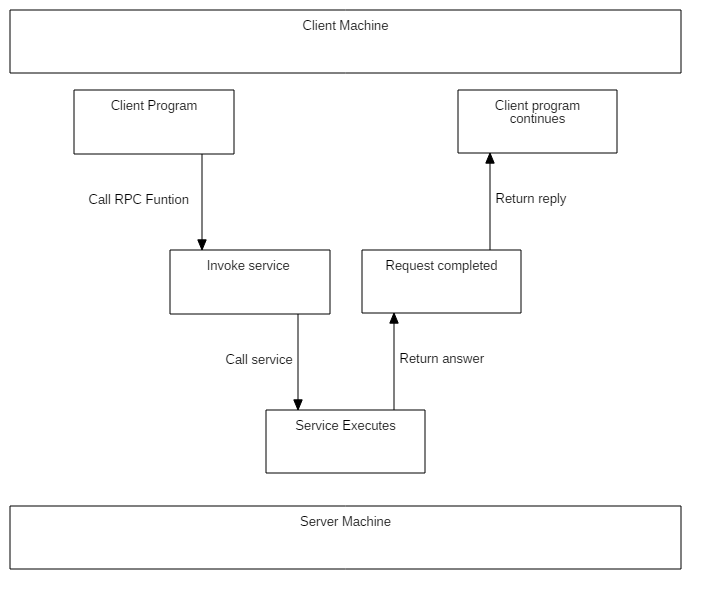
\includegraphics[width=\linewidth]{RPC.png}
\caption{System Orgranization}
\end{figure}
\section{Implement The File Transfer}
\subsection*{$server$}
\lstinputlisting[language=C]{
square_out *squareproc_1_svc(square_in *inp,struct svc_req *rqstp)
{
    static square_out out;
    out.res1= inp->arg1 * inp->arg1;
   return(&out);
}
}
\subsection*{$client$}
\lstinputlisting[language=C]{
CLIENT *cl;
square_in in;
square_out *outp;
f(argc!=3)
    {
          printf("\n\n error:insufficient arguments!!!");
          exit(-1);
    }

cl=clnt_create(argv[1],SQUARE_PROG,SQUARE_VERS,"tcp");
in.arg1=atol(argv[2]);

    if(cl==NULL)
    {
          printf("\nerror:%s",strerror(errno));
          exit(-1);
    }

    if((outp=squareproc_1(&in,cl))==NULL)
    {
          printf("\nerror :%s",clnt_sperror(cl,argv[1]));
          exit(-1);
    }
   else {
    printf("\n\n result is : %ld",outp->res1);
    exit(0);
}

(file x-square.x)
struct square_in {
   long arg1;
};

struct square_out {
 /*op result*/
 long res1;
};

program SQUARE_PROG {
version SQUARE_VERS {
    square_out SQUAREPROC(square_in)=1; /*proc no=1*/
   }=1; /*version no*/
}
}
\section{Who did what?}
- Code implement: Trinh Hoang Hai\\
- Report: Trinh Hoang Hai, Kieu Quoc Viet
\end{document}